\documentclass[12pt]{article}
\usepackage[margin=1in]{geometry}
\usepackage{setspace}
\doublespacing
\usepackage{graphicx}
\usepackage{float}
\usepackage{hyperref}
\usepackage{amsmath}
\usepackage{amssymb}

\title{From Chaos to Order\\
       \large The Fractal Geometry of Our World}
\author{Hishmat (Hish) Salehi \\
\href{mailto:hishmat@ualberta.ca}{hishmat@ualberta.ca}: 1812352}
\date{\today}

\begin{document}

\maketitle

\begin{center}
\textbf{Math/STAT 900: Capstone Project Report}  \\
\emph{Supervised by Professor Michael Y Li - 
\href{mailto:myli@ualberta.ca}{myli@ualberta.ca}}  \\
University of Alberta \\
Mathematics \& Statistical Sciences
\end{center}

\begin{abstract}
This paper is the result of my burning curiosity about Chaos Theory and Fractals and acts as an introduction to both, in hopes that it sparks some curiosity for you as well. I aim to explore the fascinating connection between Chaos Theory and Fractal Geometry in nature. 

I will begin by providing the background you will need to understand the mathematics involved to follow along. Then, I will demonstrate the incredible power of mathematics to understand the complexities of the natural world, illustrated by the complex patterns we see in coastlines, trees, and mountains. I will conclude the paper with some philosophical insights—that there is no order without chaos—and two perspectives to consider when reflecting on the unpredictable beauty of nature.
\end{abstract}

\newpage

\tableofcontents

\section{Background}


\subsection{Functions and Systems}
A function is a mathematical rule that assigns each input exactly one output. Functions are foundational in describing relationships between variables. For example, \( f(x) = x + 2 \) maps the input \( x = 3 \) to the output \( f(3) = 5 \).

A system, in this context, refers to a collection of functions and equations that interact with each other. Systems can range from simple pairs of equations to highly complex networks like weather patterns, where variables such as temperature, humidity, and wind interact dynamically.

\subsection{Deterministic and Complex Systems}
A deterministic system operates under precise rules, meaning that given an initial state, its future behavior can be predicted exactly. Classical mechanics, which governs the motion of planets and pendulums, is an example of deterministic systems.

In contrast, complex systems consist of numerous interconnected components whose interactions lead to emergent behavior that is difficult to predict. These systems exhibit properties such as nonlinearity and feedback loops, making their long-term behavior hard to forecast.

\section{Introduction}


\subsection{Chaos Theory}
Chaos theory is the study of complex systems that appear random, but in reality are governed by underlying deterministic laws. This means that even though their behavior seems unpredictable, it's driven by precise rules. The key feature of chaos is "sensitivity to initial conditions," meaning tiny changes at the start can lead to vastly different outcomes. This phenomenon is also known as the "butterfly effect."

\subsection{The Butterfly Effect}
The butterfly effect is the idea that small actions, like the flap of a butterfly’s wings, can cause large, unexpected changes, like altering weather patterns far away. It shows how tiny differences in starting conditions can lead to vastly different outcomes even in a deterministic system, where a very small difference in the beginning can make predictions difficult. Mathematically, this is expressed through exponential divergence of trajectories in phase space.

\subsection{Chaos vs. Classical Mechanics}
Classical mechanics is the study of systems that behave in a predictable way, like the motion of planets or a swinging pendulum. In classical mechanics, if you know the starting conditions (like the position and speed), you can predict exactly what will happen next. Chaos Theory, on the other hand, studies systems that can’t be predicted easily, even if they follow precise rules. Small changes at the start can lead to wildly different outcomes, making long-term predictions nearly impossible.

This sensitivity to initial conditions is what sets chaotic systems apart from the predictable systems studied in classical mechanics. Chaos Theory helps us understand that just because a system has rules doesn’t mean it’s easy to predict, especially when those rules cause big changes from tiny variations.

\subsection{Attractors in Dynamical Systems}
An attractor is a pattern or path that a system’s motion tends to follow over time. In classical mechanics, an attractor can be a single point (like an object that has come to a complete stop), a closed loop (a repeating cycle), or a torus (a combination of cycles). Attractors help scientists visualize the behavior of systems and see if they tend toward stable and predictable paths.

\subsection{Strange Attractors and Chaos}
Strange attractors are a special type of attractor found in chaotic systems. Unlike traditional attractors, strange attractors create paths that are detailed and never repeat, even though they follow specific rules. The discovery of strange attractors helped scientists understand how chaotic systems can look random but still follow hidden structures. This complexity led to more questions about how these patterns could be studied and visualized.

Strange attractors reveal that even in chaotic systems, there is an underlying structure that governs their behavior. These attractors create intricate patterns that appear random at first but show order upon closer examination. A key feature of strange attractors is their self-similarity, meaning their patterns repeat at different scales. This "self-similarity" shows that chaotic systems have repeating structures, even in their randomness. These detailed patterns in strange attractors gave rise to the concept of fractals.

\section{Fractal Geometry}


\subsection{Understanding Fractals}
Fractals are complex shapes with self-similarity, meaning they look similar at different scales of magnification. This means that each part of a fractal resembles the whole, creating patterns that repeat infinitely. Fractals are used to model naturally occurring structures that are too irregular for traditional Euclidean geometry. In Chaos Theory, fractals help describe the repeating patterns and hidden structures found in chaotic systems, like strange attractors. 

\subsection{Self-Similarity in Fractals}
Self-similarity in fractals means that the same patterns repeat at different scales. No matter how much you zoom in or out, you will see similar shapes and structures. For example, the branches of a tree look like smaller versions of the entire tree, and this is a form of self-similarity. In fractals, this property shows how simple rules can create complex and repeating structures.

\subsection{Infinite Detail}
Fractals exhibit infinite detail because their patterns continue to repeat endlessly, no matter how much you zoom in. Each part of the fractal reveals smaller and smaller structures that look similar to the whole. This means you can keep exploring deeper levels of a fractal, and there will always be more intricate details to discover. This infinite complexity makes fractals useful for modeling natural systems like coastlines, mountains, and clouds.

\subsection{Benoît Mandelbrot and the Birth of Fractal Geometry}
Benoît Mandelbrot, a Polish-born French-American mathematician, is renowned for founding the field of Fractal Geometry. In 1982, Mandelbrot published his groundbreaking book, \emph{The Fractal Geometry of Nature}, which introduced the concept of fractals to a wider audience. His groundbreaking work demonstrated that many natural phenomena, such as coastlines, clouds, and mountain ranges, possess fractal characteristics. 

Mandelbrot's most famous contribution is the Mandelbrot Set, a set of complex numbers that produces a highly intricate and infinitely detailed boundary when plotted. This set not only visualizes the beauty of fractals but also provides deep insights into the behaviour of dynamical systems.

\begin{figure}[h]
\centering
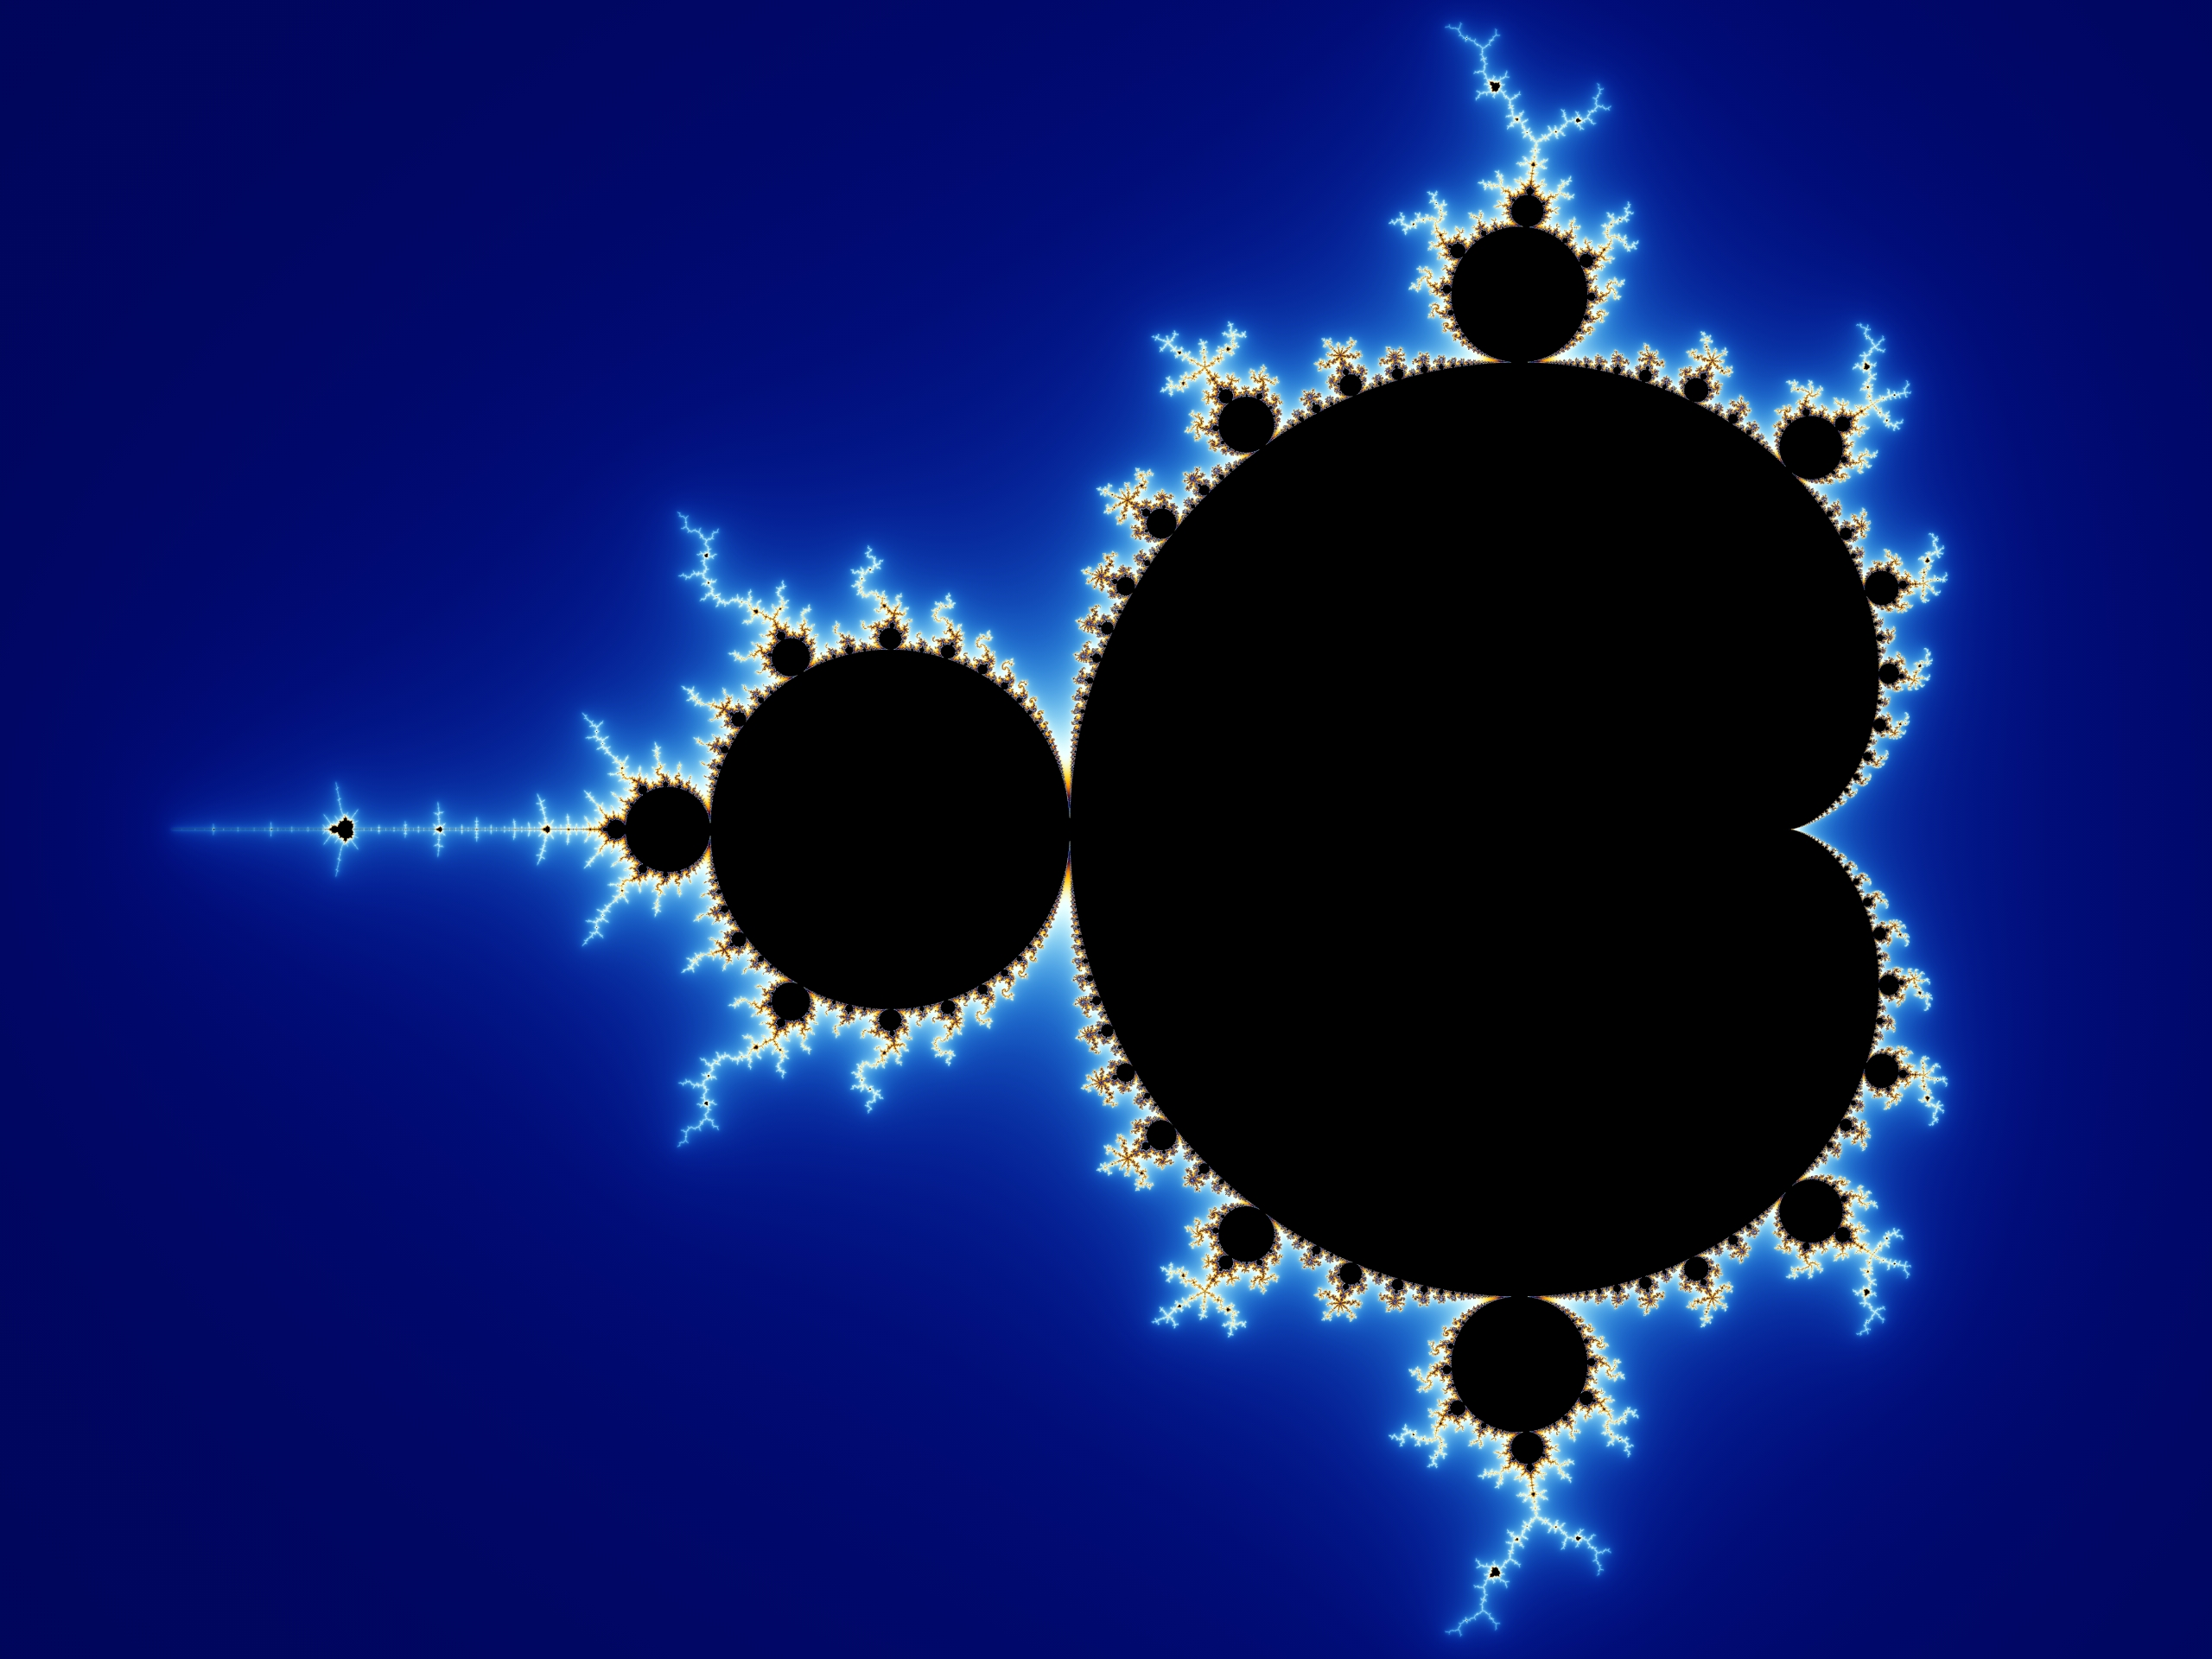
\includegraphics[width=0.5\textwidth]{assets/mandelbrot-set.jpg}
\caption{The Mandelbrot Set: A quintessential example of a fractal.}
\label{fig:mandelbrot}
\end{figure}

\section{Mathematics of Fractals and Chaos}

\subsection{The Fractal Dimension}
Fractal dimension is a way of measuring how complex a fractal is. Unlike regular shapes like lines (1D), squares (2D), or cubes (3D), fractals can have dimensions that are not whole numbers. For example, a fractal might have a dimension of 1.5, meaning it is more than a line but less than a flat surface. 

\[
D = \frac{\log(N)}{\log(1/\varepsilon)}
\]

Where \( N \) is the number of self-similar pieces, and \( \varepsilon \) is the scaling factor.

\subsubsection{Example}
For a fractal, like the Koch snowflake:
	\begin{enumerate}
		\item Divide into segments of size \(1/3\).
		\item You’ll find \(N = 4\), so \(D = \frac{\log(4)}{\log(3)} \approx 1.2619\).
		\item This non-integer dimension reflects the fractal's complexity, lying between one and two dimensions.
	\end{enumerate}
\begin{figure}[H] \centering 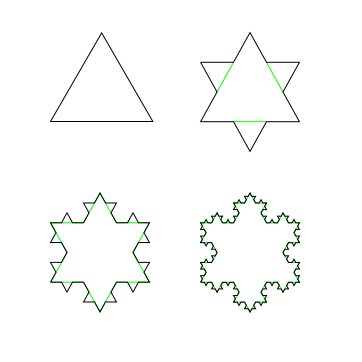
\includegraphics[width=0.36\textwidth]{assets/KochFlake.png} \caption{The first four iterations of the Koch snowflake} \label{fig:example} \end{figure}

\subsection{Iterated Function Systems (IFS)}
Iterated Function Systems are a powerful method for generating fractals through the repeated application of a finite set of contraction mappings. Each mapping transforms the fractal in a specific way, and by iterating these transformations, complex self-similar patterns emerge.

Mathematically, an IFS consists of a set of functions \( \{f_i\}_{i=1}^N \), where each \( f_i: \mathbb{R}^n \to \mathbb{R}^n \) is a contraction mapping. This means there exists a constant \( 0 \leq c < 1 \) such that for all \( x, y \in \mathbb{R}^n \),
\[
\| f_i(x) - f_i(y) \| \leq c \| x - y \|.
\]
The fractal is generated by starting with an initial shape, often called the "seed," and repeatedly applying each of the contraction mappings to this shape. Over many iterations, the combined effect of these transformations produces intricate and infinitely detailed patterns.

\subsubsection{Example: Sierpiński Triangle}
A classic example of a fractal generated by an IFS is the Sierpiński Triangle. It is constructed using three specific contraction mappings that scale and translate an initial equilateral triangle to each of its three corners.

The three contraction mappings for the Sierpiński Triangle are:
\[
f_1(x, y) = \left( \frac{x}{2}, \frac{y}{2} \right),
\]
\[
f_2(x, y) = \left( \frac{x}{2} + \frac{1}{2}, \frac{y}{2} \right),
\]
\[
f_3(x, y) = \left( \frac{x}{2} + \frac{1}{4}, \frac{y}{2} + \frac{\sqrt{3}}{4} \right).
\]

\begin{itemize}
    \item Step 1: Start with an initial point, such as \( (0,0) \).
    \item Step 2: Randomly select one of the three functions and apply it to the current point to obtain a new point.
    \item Step 3: Repeat Step 2 iteratively, plotting each new point.
\end{itemize}

After numerous iterations, the points will approximate the Sierpiński Triangle, revealing its self-similar structure. \href{https://cs.lmu.edu/~ray/notes/ifs/}{Test it out for yourself.}

\begin{figure}[h]
\centering
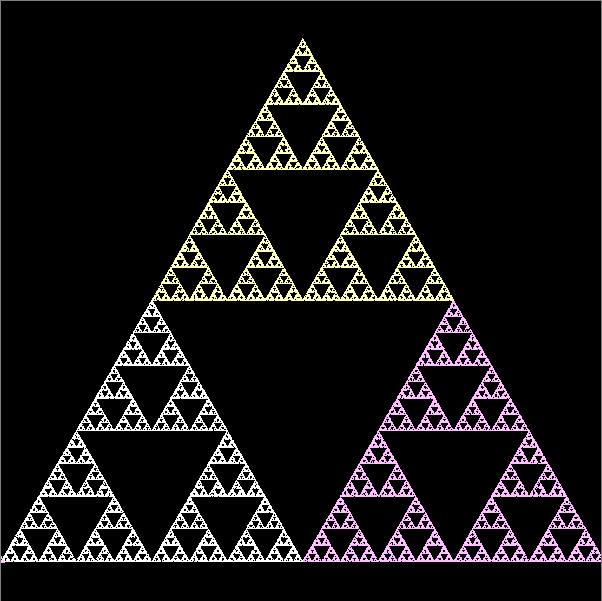
\includegraphics[width=0.5\textwidth]{assets/sierpinski-triangle.png}
\caption{Sierpiński Triangle generated using Iterated Function Systems.}
\label{fig:sierpinski}
\end{figure}

\subsection{Iterated Maps}
Iterated maps are mathematical functions applied repeatedly to a value or set of values. They are fundamental in studying dynamical systems and generating fractals. An iterated map can be expressed as:
\[
x_{n+1} = f(x_n)
\]
where \( f \) is a function defining the system's rules. For example, the logistic map is a simple iterated map given by:
\[
x_{n+1} = r x_n (1 - x_n)
\]
where \( r \) is a parameter. As \( r \) varies, the behavior of the map changes, demonstrating transitions from stable points to chaotic dynamics. Iterated maps help visualize how complex patterns and chaos emerge from simple mathematical rules.

\subsection{Lyapunov Exponents: Measuring Chaos}
Lyapunov exponents quantify the rate at which nearby trajectories in a dynamical system diverge. A positive Lyapunov exponent indicates chaos, as it signifies sensitive dependence on initial conditions. Mathematically, the Lyapunov exponent \( \lambda \) is defined as:
\[
\lambda = \lim_{t \to \infty} \frac{1}{t} \ln \frac{d(t)}{d(0)}
\]
where \( d(t) \) is the distance between two trajectories at time \( t \). If \( \lambda > 0 \), the system is chaotic, meaning that small differences in initial conditions can lead to vastly different outcomes over time. This measure is crucial for identifying and characterizing chaotic behavior in various systems, from weather patterns to financial markets.

\subsection{Bifurcation Theory and Transition to Chaos}
Bifurcation theory studies how small changes in a system's parameters can lead to sudden qualitative changes in its behavior. A common route to chaos is through period-doubling bifurcations. Consider the logistic map:
\[
x_{n+1} = r x_n (1 - x_n)
\]
As the parameter \( r \) increases, the system undergoes a series of bifurcations where the number of stable points doubles, leading from stable fixed points to periodic cycles and eventually to chaotic behavior. For instance, at \( r \approx 3.56995 \), the system transitions to chaos, exhibiting unpredictable and aperiodic behavior. Bifurcation theory helps explain how deterministic systems can become chaotic, highlighting the intricate balance between order and disorder.


\section{Fractals in Nature}
\subsection{How do chaotic processes contribute to fractal patterns in nature?}
TODO

\subsection{How do coastlines display fractal patterns?}
TODO

\subsection{How do trees display fractal patterns?}
TODO

\subsection{How do mountains display fractal patterns?}
TODO

\section{Conclusion}

The dynamics of a system at each moment of time can be in one of these two states:
\begin{itemize}
    \item Chaos (unstable)
    \item Order (stable)
\end{itemize}


At either of those states you also need a perspective to be able to maximize your effectiveness and live optimally. These perspectives are Zooming out and Zooming in. 

You zoom out when the system is in a state of chaos. What that means is you try to grasp the bigger picture and understand why things unfold in the long run.

You zoom in when the system is in a state of order. What that means is you bring yourself to the present moment and try to take it in as much as possible. This includes when the economy is stable, when routines are predictable, and when life feels steady.

Chaos theory teaches us that there is no certainty in life, only possibility and patterns, and that is enough.


\nocite{*} 
\bibliographystyle{plain} 
\bibliography{references}

\end{document}
